\documentclass[a4paper,12pt]{article}


\usepackage{amsmath}
\usepackage[english]{babel}
\usepackage[utf8]{inputenc}
%\usepackage[ascii]{inputenc}
\usepackage{amssymb}
\usepackage{graphicx}
\usepackage{varioref}
\usepackage{siunitx}
%\usepackage[margin=.9in]{geometry}
\usepackage[a4paper, top=2cm, bottom=2cm, left=2.5cm, right=1cm]{geometry}
\usepackage{abstract}
\usepackage[T1]{fontenc}
%\usepackage{float}
\usepackage[english]{babel}
\usepackage{fancyhdr}		% for headers

\usepackage{url}
\usepackage{hyperref}
\usepackage[hypcap=true]{caption}

%appendix
\usepackage[title,titletoc,toc]{appendix}

%***************** Packages for Graphics & Figures *******************%
\usepackage{graphicx} %%For loading graphic files
\graphicspath{ {images/} } %graphics path located inside image folder
%*******************************************************************%

\fancyhf{}
\fancyhead[l]{CS671 ICT for Socio Economic Development Project Report, CSE Dept, IIT Bombay, April,2017 (Course Instructor - Prof. Krithi Ramaritham )}
\fancyfoot[c]{\thepage}

\pagestyle{fancy}

% % convert plain page style to fancy on title page
\makeatletter
\let\ps@plain\ps@fancy 
\makeatother


\begin{document}
\begin{titlepage}

\end{titlepage}
%opening
\title
	{
		Air Quality Monitoring
	}
\author
	{
		Parin Chheda (153076005) parin[at]ee.iitb.ac.in\\
		Naveen (15305R005) naveendotc[at]cse.iitb.ac.in	\\
		Saurav Shandilya (153076004) shandilya[at]ee.iitb.ac.in
	}

\maketitle


\section{Introduction}
Air pollution is a serious issue in urban cities. The deteriorating air quality is a cause of a plethora of heart and lung diseases. Burning of wood/plastic waste, Metal processing plants, vehicular emissions are the major sources of air pollutants. These pollutants are referred to as “Particulate Matter“ as they remain suspended in air and can enter human lungs while breathing. PM 2.5 (Particulate Matter) (2.5 microns) is categorized worldwide to be the major cause of respiratory and cardiovascular problems. Apart from this other pollutants like Carbon Monoxide (CO), Sulphur dioxide SO$_2$, PM 10 etc also affect human health when present in significant quantities.\cite{report_shubham}
\newline
Statistical data about the concentration of air pollutants in different parts of the city can assist in the following ways:
\begin{itemize}
\item Help to locate the source of emissions.
The policy makers of the city can impose restrictions in case it is an industry/factory to reduce emissions. 
\item Data driven decisions can be taken by policy makers.
The correlation between the data collected about the air quality and the diseases prevalent in an area can detect early onset of diseases.
\item Create awareness among citizens
\end{itemize}
The commercially available Particulate matter sensors like Dylos 1100 C Pro (Cost: 300\$) and SDS 011 (Cost: 40 \$) are expensive with high power consumption. On the other hand there are sensors like Samyoung DSM 501 A (Cost: 12\$) and Shinyei PPD42Ns (Cost: 10\$) which claim to sense PM 2.5 using LED/photodiode arrangement with moderate accuracy. 
Using low cost sensors to sense PM 2.5 levels in windowed thresholds if not as accurately as the commercially avialable ones can be a stepping stone in monitoring air quality of different city areas.
Battery powered sensor nodes with low cost sensors and solar charging capability will be an optimum solution to address the issue of monitoring air quality at relatively lower budget. 

To visualize all these data collected, we need some kind of interface using which we can analyse and draw some very useful conclusions like what are the causes for the pollution levels going high or low. Also we can compare the pollution levels at various junctions of the city and we can take necessary measures to maintain the pollution levels with in limit. There are few interfaces online which shows the live data of pollution levels but they are lagging in the user interaction experience. Although they are data available, sufficient analytics was not done to draw useful conclusions. As we know, having large data set with no analytics behind doesn't make any sense to the data. So we are planned to have user friendly interface with sufficient backend data analytics.   

\section{Problem definition}
Design a sensor node with air quality, temperature and humidity sensors and display it on a visualization tool to interpret them. Air Quality Monitoring requires measurement of eight pollutants, viz. PM10, PM2.5, NO$_2$, SO$_2$, CO, O$_3$, NH$_3$, and Pb.
However, tracking PM 2.5 levels as started by \textbf{SAFAR} Project \cite{safar} and \textbf{breathe} \cite{breathe} is essential to estimate air quality.
In this project we are trying to do the following:
\begin{itemize}
\item Build a low cost-low power sensor node with CO, temperature, Humidity and PM 2.5 sensors.
\item Exploring the alternative of low cost sensors as a replacement for high cost ones.
\item Design a stackable sensor node which provide feature to easily add/remove sensors as required  
\item Visualizing the data received from the sensors for better visualization.
\end{itemize}
From the data that we received from the sensor node, we had the following  analytics:
\begin{itemize}
\item Live data of the sensor node which includes temperature, humidity, PM 2.5, Co levels.
\item Hourly average of temperature, humidity, PM 2.5, Co levels for the past few days(currently fixed it for past 2 days).
\item Hourly average of all the above parameters in between the queried period.
\item Complete data of the current date.
\end{itemize}

System architecture of our solution is shown in Figure \ref{fig:sys_arch} 
\begin{figure}[!ht]
	\centering
	\includegraphics[scale=0.5]{system_archi1.jpg}
	\caption{System Architecture}
	\label{fig:sys_arch}
\end{figure}

\section{Requirements}
\subsection{Hardware Requirements}
Sensor node and the central server present the major hardware requirement.
%\newline Sensors :
\begin{itemize}
\item Sensors
\begin{itemize}
\item MQ-7 - Carbon monoxide (CO) \cite{co_datasheet}
\item DSM 501A - Particulate matter (PM2.5) \cite{dsm_datasheet}
\item DHT22 - Temperature and Humidity Sensor \cite{dht22_datasheet}
\end{itemize}
\item Controllers
\begin{itemize}
\item MSP430F5529 Launchpad - for sensor node
\item Raspberry Pi (2, Model-B) - as data and web server
\end{itemize}
\item Communication Module
\begin{itemize}
\item CC2530 Zigbee (IEEE 802.15.4)
\end{itemize}
\item Sensor Node Design
\begin{itemize}
\item Stackable Headers and general purpose perforated boards
\item MOSFET switches : PSMN022-30pl (N type Enhancement mode)
\item Battery : Lithium Ion (3.7V, 2600mAH)
\item CN6009 Boost Converter (3.7V to 5V)
\item Indicator LEDs, Push-to-on switches, connectors
\item Discrete resistors

\end{itemize}
\end{itemize}
\subsection{Software Requirements}
\begin{itemize}
	\item Django 1.10
    \item plot.ly Javascript library
    \item Sqlite3
    \item PyCharm
    \item Energia and Code Composer Studio
\end{itemize}
\section{Real world issues and considerations / assumptions}
% Functionality: Inputs, outputs and constraints
\label{sec: Issues and Calibration}
 
\subsection{Sensors : Calibration and inherent constraints}
\subsection*{MQ-7 CO(Carbon monoxide)}
\subsubsection{Description}
MQ-7 is a chemical sensor which is sensitive to CO, H$_2$, alcohol and LPG. The sensor has a heater element and uses heat as a catalyst to vary the resistance of its sensing film based on gas concentration.
\\
Range of CO sensor is 20-2000 ppm
\subsubsection{Calibration}
The output of the sensor is change in resistance of its sensitive film due to a change in concentration of the above mentioned gases. The figure\ref{fig:temp1} below shows the resistance ratio \textbf{(RS/Ro)}
% * <kevinjoshi9888@yahoo.co.in> 2017-04-24T12:16:17.591Z:
% 
% > The output of the sensor change in resistance of its sensitive film due to a change in concentration of the above mentioned gases.
% 
% Rephrase.
% 
% 
% ^.
where \textbf{'RS'} is the sensor or film resistance and \textbf{'RO'} is the sensor resistance in clean air.
\begin{figure} [!ht]
\centering
\includegraphics[scale=0.5]{MQ_7.png}
\caption{MQ 7 Output characteristics}
\label{fig:temp1}
\end{figure}
\subsubsection{Curve fitting}
The first step in calibrating the sensor was to find out the output function i.e. equation for ppm given the RS/RO ratio. We got following function after curve fitting.
\begin{equation}
f(x) = 1534x^-0.216 - 1350
\hspace{0.5cm} \textnormal{where x is RS/Ro}
% * <kevinjoshi9888@yahoo.co.in> 2017-04-24T12:17:27.017Z:
% 
% > f(x) = 0.02791x^2 + 614.1x + 4.921
% 
% Accuracy of fit ?
% 
% ^.
\end{equation}
\\The above power function gives an R2 of about 0.97
\\
 The concentration of CO in clean air or indoor environment is between 1-4 ppm. However our sensor has a range of 20-200 ppm. However due to our calibration or curve fitting function, it shows 1-3 ppm in indoor environment.While, computing the curve fit an assumption of 2 ppm of CO in air was taken.
\subsection{DSM 501 A (Particulate Matter or Dust Sensor)}
% * <kevinjoshi9888@yahoo.co.in> 2017-04-24T12:15:53.789Z:
% 
% Sensor resolution?
% 
% ^.
\subsubsection{Description} 
The sensor works on counting the number of particles in the air passing through it i.e. opacity of air using Led and Photo detector module. The sensor characteristics given in the data sheet does not present the amount of granularity as required to come up with a good curve fit.
\\
Maximum concentration measurable by PM 2.5 sensor is 15,000 pcs/283ml

\subsubsection{Calibration}
The sensor gives a PWM output in response to detection of dust particles. The output goes low for a duration proportional to the concentration of dust particles. The sensor gives two outputs:
\newline \textbf{Vout2} : Gives concentration of particles above \SI{1}{\micro\metre}.
\newline \textbf{Vout1} : Gives concentration of particles above \SI{2.5}{\micro\metre}.
\newline A sample PWM output from the sensor is shown in \ref{fig:temp2}. The data sheet shows two interesting graphs one \textbf{Low ratio\% vs particle in milligram/m3} and second one is\textbf{ Low ratio\% vs particles(pcs)/283ml}. After verifying experimentally and comparing with Dylos Sensor, we found that the second graph is more useful and possibly more accurate. This graph is shown in \ref{fig:temp3}. According to this graph, we choose to fit the sensor output values to a fitting function using Matlab. We got the following function for pcs/283ml vs Low ratio\%.
\begin{equation}
f(x) = 0.02791x^2 + 614.1x + 4.921
\hspace{0.5cm} \textnormal{where x is Low ratio\%}
% * <kevinjoshi9888@yahoo.co.in> 2017-04-24T12:17:27.017Z:
% 
% > f(x) = 0.02791x^2 + 614.1x + 4.921
% 
% Accuracy of fit ?
% 
% ^.
\end{equation}
This polynomial function gives an R2 of about 0.997.
\\
\newline
The figure\ref{fig:dsm_out_char} shows the plot of the fitted function versus sensor response taken from the data sheet.The pcs/283ml is equivalent to pcs/0.01 cubicfoot. The Dylos sensor against which we tried to correlate always gives the output in the same unit.
\subsubsection{Interfacing}
The \textbf{Vout2} and \textbf{Vout1} PWM outputs are connected to digital I/O pins on the micro controller. We check the duration of low pulse in a time window of 30 seconds to determine the Low ratio\%. The computation of f(x) i.e. concentration in pcs/0.01 cubicfoot is done on the server.

\begin{figure}[!ht]
\centering
\includegraphics[scale=0.5]{dsm_3.png}
\caption{Curve fit}
\label{fig:temp3}
\end{figure}

\begin{figure}[!ht]
\centering
\includegraphics[scale=0.5]{dsm_1.png}
\caption{DSM 501 A Sample Output}
\label{fig:temp2}
\end{figure}

\begin{figure}[!ht]
\centering
\includegraphics[scale=0.5]{dsm_2.png}
\caption{DSM 501 A Output Characteristics }
%\label{fig:temp3}
\label{fig:dsm_out_char}
\end{figure}

\subsection{DHT 22 (Temperature and Humidity Sensor)}
\subsubsection{Description} 
Uses capacitive humidity sensing and thermistor for temperature sensing \cite{dht22_datasheet}. The sensor comes precalibrated and outputs digital temperature and relative humidity percentage on a single wire. \\

Operating range of Temperature sensor is -40ºC to 80ºC \\
Operating range of Humidity sensor is 0-100\%RH \\
Resolution of Temperature sensor is $\pm$ 0.1ºC \\
Resolution of Humidity sensor is $\pm $ 0.1\%RH


\subsubsection{Calibration}
Since the sensor comes precalibrated, we decided to test its performance against another precalibrated weather monitoring station (Netatmo). 
\newline
The figure \emph{\ref{fig:temp}} shows the plot of temperatures sensed by the two over a span of three hours. We provided a step input by turning ON the air conditioner at around 4:20 am. From the plot, it can be seen that DHT22 is sluggish and has a higher response time as compared to Netatmo. However, DHT22 catches up with Netatmo as soon as temperature becomes relatively stable.
\begin{figure}[!ht]
\centering
\includegraphics[scale=0.5]{dht_temp.jpg}
\caption{DHT22 Temperature vs Netatmo}
\label{fig:temp}
\end{figure}

\paragraph*{}
Next, we compared the humidity readings between the two. As it can be seen from the plot \ref{fig:hum} DHT22 is more sensitive to humidity changes and shows an average error or difference of
3.648\%. Surprisingly the humidity levels do not go down when air conditioner is switched ON.
\begin{figure}[!ht]
\centering
\includegraphics[scale=0.5]{dht_humdity.png}
\caption{DHT22 Humidity vs Netatmo}
\label{fig:hum}
\end{figure}

\subsection{Challenges Faced}

\begin{itemize}
\item Low Power Optimization: Initial objective of project was to make the whole system low power and make it sustain itself on a 3.3V battery. However the CO sensor we used required a heater operating at 5V. This heater consumed substantial amount of current during battery operation. Hence low power operation was not possible.

\item Sensor Switching: We used MOSFETs switches to turn OFF sensor when not in use. Individually, we were able to switch them ON/OFF, however when placed on the stack, we found that sensors dont switch ON once off or switch off once ON. While debugging we found a solution to this which is to have a separate ground path for DSM 501 A and MQ-7. But since the board was already made, we didi not change the connections, however we tested this out by placing the assembly on the breaboard.

\item Zigbee Communication: Communication between central server and multiple sensor node. With multiple sensor node, we faced issue of data packet loss and intermixing of data from several nodes.

\item Sensor Calibration: Since the datasheet did not present the information about sensor reponse in the granularity desired, several problems and confusions occured while interfacing them.

Resolution: We handled the problem through software. Each sensor node is assigned a id and a count (number of sensors connected to node) from admin page of website at time of commissioning (refer figure \ref{admin}). Sensor nodes are in sleep mode to reduce power consumption. Central server broadcast wakeup signal and nodeid. This wakeup the sensor node and if nodeid matches that of sensor node, data is transmitted as per format specified. Central server request data from sensor nodes in sequential order, thus preventing the intermixing of data. To resolve issue of data loss, we tried a basic resolution of matching the data packet length and if mismatch is found, data is retransmitted. Implementing a CRC resolves the issue completely.

Another issue we faced with CC2530 hardware module was issue of module transmitting random data continuously. In order to resolve the issue, We tested short of Tx pin of CC2530 pins and attached a external pullup resistor. These method did not helped us and we hence can not make the module work. This caused a major limitation in development as we can not create a second sensor node.  



\item Finding the suitable library for live data plotting, also suitable web-server for Raspberry PI is definitely a challenge.
\item The web-server and database server are both running on Raspberry Pi, there is need of optimizing the response time of the web-interface.
\item Bootstrap is a CSS and javascript framework which helps in reducing the response time as there is no need for user to load these script files from the server(Raspberry Pi) instead these can be loaded from CDN. If at all these are loaded from server then load on server is increase alot which ultimately increases the response time.
\item As it is known that Django is a developer friendly environment, but for a beginner who is very new to MVC framework it's really a challenge to build a user friendly environment within a limited time.

\end{itemize}


\section{Test results}
\label{sec:Test_result}
We developed both the software and hardware modules simultaneously. During the initial stages of the project as we don't have the real time data, we generated the random data using python. Later we decided to change the way the random data is generated. This is because the data is generated randomly irrespective of the time stamp i.e., temperature at 2 PM can even be 10 degree centigrade(considering climate at IIT Bombay) which is not the correct way. Later we moved to other way of generating the random data i.e., through XL sheet. This generates the data depending on the time stamp which is a good idea to proceed with. We finally tested the web application using this generated data.
\subsection{Testing MQ7 (Carbon Monoxide sensor)}
The resistance measured from this sensor varied with exposure to candle. The ppm output showed some changes, but not precise as such a small CO concentration is outside its measurement range.
\subsection{Testing DHT22 (Temperature and Humidity sensor)}
The readings from DHT22 were compared against a precalibrated Netatmo sensor. The results are included in our presentation.
\subsection{Testing DSM 501 (Particulate matter sensor)}
We tried to see the correlation between our dust sensor and the commercially available Dylos 1100C Pro Sensor.
\newline \textbf{Test-1}: We only took the \textbf{Vout2} i.e. particle concentration above \SI{1}{\micro\metre}. The location was KReSIT terrace.
\begin{figure}[!ht]
	\centering
	\includegraphics[scale=0.5]{dsm_test_1.png}
	\caption{Test-1 Results}
	\label{fig:test1}
\end{figure}
\newline\textbf{Test-2} : Since we did not see much correlation, we took both the \textbf{Vout1} and \textbf{Vout2} readings subtracted them as the result should theoretically give PM \SI{2.5}{\micro\metre} levels. The location for the test was Gulmohar hotel compound just besides a moderately busy road.The peak in levels of Dylos between 8:20 to 8:30 pm shown in \ref{fig:test2} was due to a procession with many people along with trucks passing by.
\begin{figure}[!ht]
	\centering
	\includegraphics[scale=0.5]{dsm_test_2.png}
	\caption{Test-2 Results}
	\label{fig:test2}
\end{figure}
\newline\textbf{Test-3} : For this test, we placed both the Dylos and our dust sensor indoors where the levels of particulate matter are low and do not change much.The results of the test is plotted in \ref{fig:test3}. \\

\begin{figure}[!ht]
	\centering
	\includegraphics[scale=0.5]{dsm_test_3.png}
	\caption{Test-3 Results}
	\label{fig:test3}
\end{figure}

\textbf{Miscellaneous} : As per the Air quality standards (AQI) in India, the PM 2.5 levels are specified in \SI{}{\micro\gram}/m3. The University of Montana's Center for Environmental Health Sciences came up with a conversion function for translating pcs/0.01 cubic foot to \SI{}{\micro\gram}/m3. Using this function \cite{dylos}, we have plotted PM 2.5 levels from the data accumulated in Test-2. 
\begin{figure}[!ht]
	\centering
	\includegraphics[scale=0.5]{dsm_test_4.png}
	\caption{PM 2.5 levels in \SI{}{\micro\gram}/m3}
	\label{fig:test4}
\end{figure}
\newline observations : We found that DSM 501 A is quite noisy. However, if we use a simple 3 point moving average filter as shown in \ref{fig:test4} we can reduce noise to some extent. If we look at the plot in \ref{fig:test4} carefully, the trend of DSM 501 A readings starts increasing at 8:30, but at slower pace as compared to Dylos. Also in all the graphs, we see that there is an offset of the order of 1000 pcs/0.01 cubic foot or 5\SI{}{\micro\gram}/m3. 
\newline In all these tests, the readings were taken at 1 minute intervals for about an hour. Now if we take hourly average of the values obtained (Since hourly averages are mostly displayed on air quality monitoring sites)

% Test-2 : 
% Dylos 1100C Pro 1 Hour average : 5082 pcs/0.01 cubicfoot, \SI{34}{\micro\gram}/m3
% DSM 501A 1 Hour average : 2447 pcs/0.01 cubicfoot, \SI{15}{\micro\gram}/m3

% Test-3 :
% Dylos 1100C Pro 1 Hour average : 3783 pcs/0.01 cubicfoot ,\SI{26}{\micro\gram}/m3
% DSM 501 A 1 Hour average : 2802 pcs/0.01 cubicfoot,\SI{19}{\micro\gram}/m3

\begin{table*}[!ht]

\label{table_1}
\centering
\begin{tabular}{|l|l|l|l|l|}
\hline
\bfseries Test no. & \multicolumn{2}{c}{\bfseries Dylos 1100C} \vline & \multicolumn{2}{c}{\bfseries DSM501A} \vline \\
\hline
& pcs 0.01/cu.ft. & ug/m3 & pcs 0.01/cu.ft. & ug/m3\\
\hline
2 & 5082 & 34 & 2447 & 15\\
\hline
3 & 3783 & 26 & 2802 & 19 \\
\hline

\end{tabular}
\caption{PM2.5 data comparison between Dylos and DSM}
\end{table*}

DSM 501 A performs better and readings correlate better, if dust concentration is almost constant as in case of Test-3 in indoor conditions. However for outdoor conditions, more tests need to be performed to find out offset to be added and evaluate performance of DSM 501 A in terms of giving results in windowed thresholds often required to estimate air quality.\cite{PM}

\begin{figure}[!ht]
	\centering
	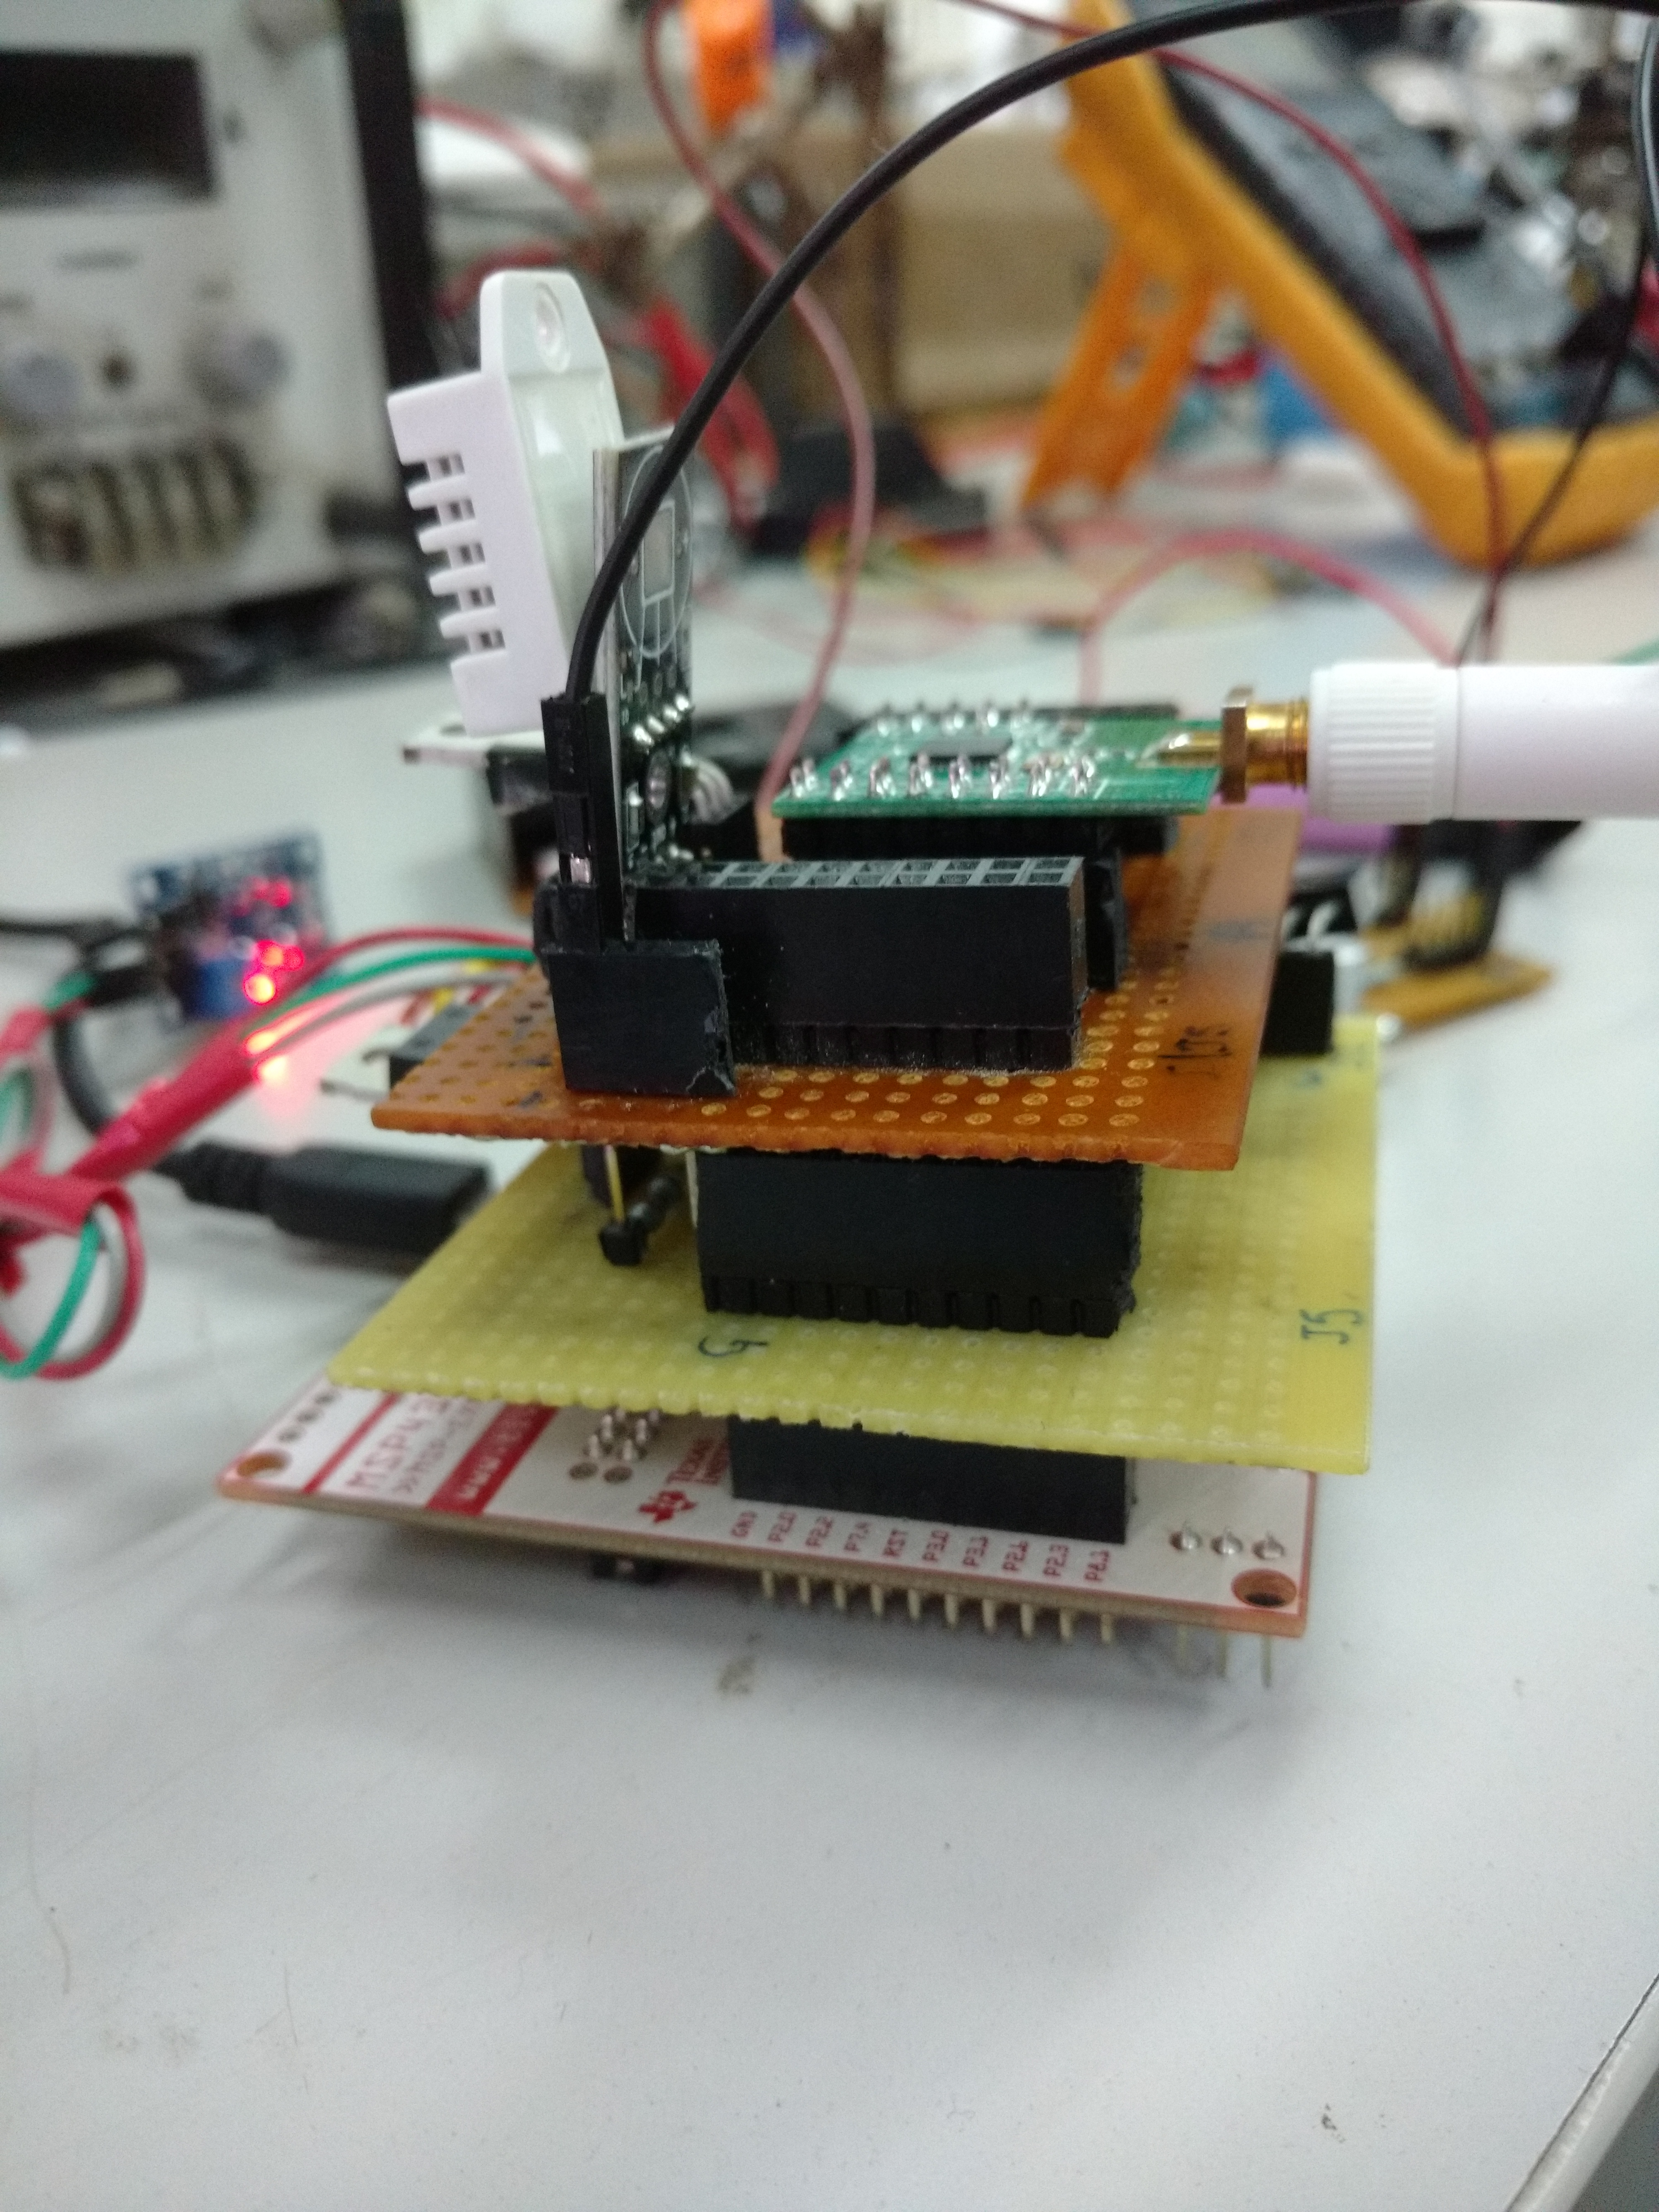
\includegraphics[width=400pt,height=350pt]{stack.jpg}
	\caption{Stack Design}
	\label{fig:stack}
\end{figure}

\subsection{Stack Design}
Figure \ref{fig:stack} shows sensor stacks and its mounting on controller board. We had designed two stacks. One stack contains DHT22 sensor and other stack has MQ7 and DSM sensors.

\subsection{Data Analysis Plots from Web Interface}
The library which was used to plot these is plotly javascript\cite{Plotly}. The figure \ref{live} shows the live data of a particular sensor which is installed at ERTS lab. Live data shows temperature, humidity, CO levels and PM2.5. 
\begin{figure}[!ht]
	\centering
	\includegraphics[width=500pt,height=350pt]{live.png}
	\caption{Live data displayed on marker}
	\label{live}
\end{figure}
The figure shown in \ref{co} shows the hourly average of CO levels in between a customized period. We have added color codes to the CO and PM2.5 levels but as we have measured this lab we couldn't get the data for all levels of CO.
\begin{figure}[!ht]
	\centering
	\includegraphics[scale=0.5]{co.png}
	\caption{Hourly Average of CO Levels}
	\label{co}
\end{figure}
The figure shown in \ref{temp1} shows hourly average of temperature in between customized period. The figure shows data of 17th and 18th April 2017.
\begin{figure}[!ht]
	\centering
	\includegraphics[scale=0.5]{temp1.png}
	\caption{Hourly Average of Temperature in degree centigrade}
	\label{temp1}
\end{figure}
The figure shown in \ref{temperature} shows hourly average of temperature on a particular day. The figure shows data of 17th April 2017.
\begin{figure}[!ht]
	\centering
	\includegraphics[scale=0.5]{temperature.png}
	\caption{Hourly Average of Temperature in degree centigrade}
	\label{temperature}
\end{figure}

\begin{figure}[!ht]
	\centering
	\includegraphics[scale=0.5]{adminpage.png}
	\caption{Admin can add a new marker when a new sensor node is installed\cite{Django}}
	\label{admin}
\end{figure}

The interface which we developed is scalable in the sense that in future if we add any new sensor node to it, it starts receiving the live data. The only thing that we need to do is add the node marker with its location attributes(latitude and longitude). The figure shown in \ref{admin} displays how to add a new marker(location of sensor node) to the Google API. When a new sensor node is added in the network, a id is assigned to it. This id is used for identification of several several nodes.


\newpage
\section{Conclusion}

The aim of the project was to develop a low power, low cost, wireless sensor nodes to measure air quality with objective to have a stackable design of sensor node. 

We successfully interfaced sensors as per plan. We calibrated the sensors and performed various tests to compare value of sensors we used with standard sensors. We discussed our findings and test results in section \ref{sec: Issues and Calibration} and section \ref{sec:Test_result}. Web interface for data visualization is done and discussed in section \ref{sec:Test_result}.

This project has following scope of future development and improvement:
\begin{itemize}
\item Trying other sensors
\item Due to issue faced with Zigbee module (discussed in section \ref{sec: Issues and Calibration}), we could not efficiently test working of multiple sensor nodes. Testing can be done on different zigbee module
\item Improving response time and UI of web interface

\end{itemize}


\bibliographystyle{unsrt}
\newpage
\bibliography{aqm_reference}

\newpage

\appendix
\begin{center}
\section{Appendix}
\end{center}

\subsection{Circuit Connections}
The circuit consist for sensors, communication module, power unit, microcontroller and raspberry pi. This section shows connection of each of the components. Power to each sensor is controlled through MOSFET switch. MOSFET gate is controlled though IO pin of microcontroller and it is used to cuts the power supply of sensor during idle state, thus saving the power. Figure~\ref{fig:msp430_conn} shows connections on MSP430. Figure~\ref{fig:pi_conn} shows connections on Raspberry Pi and 

\begin{figure} [!ht]
	\centering
	\includegraphics[scale=0.25]{msp430.png}
	\caption{MSP430F5529 connections}
	\label{fig:msp430_conn}
\end{figure}

\begin{figure}[!ht]
	\centering
	\includegraphics[scale=0.35]{pi.png}
	\caption{Raspberry Pi connections}
	\label{fig:pi_conn}
\end{figure}

\begin{figure}[!ht]
	\centering
	\includegraphics[scale=0.4]{boost.png}
	\caption{3.3V to 5V boost converter connections}
	\label{fig:boost_conn}
\end{figure}

\subsubsection{DHT 22 Connections}
Figure~\ref{fig:dht22_conn} shows connection for DHT22 (Temperature and Humidity sensor). Sensor has 3 pins viz. Ground, V$_{cc}$ and Signal(V$_o$). Sensor is powered on 3.3V voltage rail. Sensor provided a digital output on single wire. Signal pin is connected to Port2 pin0 of micro-controller as shown in Figure~\ref{fig:msp430_conn}. Port1 pin5 is connected to gate of MOSFET for sensor switching.

\begin{figure}[!ht]
	\centering
	\includegraphics[scale=0.25]{temp.png}
	\caption{DHT22 (Temp. and Humidity) sensor connections}
	\label{fig:dht22_conn}
\end{figure}

\subsubsection{DSM 501 Connections}
Figure~\ref{fig:pm2_5_conn} shows connection for DSM 501 (Particulate Matter sensor). Sensor is powered on 5V voltage rail. Sensor provided a PWM output on two pins which are connected to Port4 pin1 and Port4 pin2 of micro-controller as shown in Figure~\ref{fig:msp430_conn}. Port3 pin6 is connected to gate of MOSFET for sensor switching.

\begin{figure}[!ht]
	\centering
	\includegraphics[scale=0.25]{pm2_5.png}
	\caption{DSM501A (PM-2.5) sensor connections}
	\label{fig:pm2_5_conn}
\end{figure}


\subsubsection{MQ7 Connections}
Figure~\ref{fig:co_conn} shows connection for MQ7 (Carbon Monoxide sensor). Sensor is powered on 5V voltage rail. Sensor provided analog output on and is connected to Port6 pin0 of micro-controller as shown in Figure~\ref{fig:msp430_conn}. Port2 pin5 is connected to gate of MOSFET for sensor switching.

\begin{figure}[!ht]
	\centering
	\includegraphics[scale=0.25]{CO_circuit.png}
	\caption{MQ7 (Carbon Monoxide) sensor connections}
	\label{fig:co_conn}
\end{figure}

\begin{figure}[!ht]
	\centering
	\includegraphics[scale=0.4]{cc2530.png}
	\caption{CC2530 (Zigbee Module) connections}
	\label{fig:cc2530_conn}
\end{figure}

\subsubsection{CC2530 Connections}
Figure~\ref{fig:cc2530_conn} shows connection for CC2530 (Zigbee based connection module). It is powered on 3.3V voltage rail. It is interfaced on serial(UART). 

Zigbee module is connected to microcontroller. It is responsible for sending the sensors data. It is connected to Port3 pin3 and Port3 pin4 of micro-controller as shown in Figure~\ref{fig:msp430_conn}. 

A zigbee coordinator is connected to Raspberry Pi. Coordinator is responsible to get sensor data. Data is stored in database and displayed on website. It is connected to Pin8 and Pin10 of Raspberry Pi as shown in Figure~\ref{fig:pi_conn}.





\end{document}
